% Chapter 8

\chapter{Integration of DJANGOH in the Monte-Carlo Chain} % Chapter title

\label{ch:MC} % For referencing the chapter elsewhere, use \autoref{ch:name}

%----------------------------------------------------------------------------------------

\section{TGEANT}


%----------------------------------------------------------------------------------------

\section{DJANGOH as a physics generator for TGEANT}

The original DJANGOH is a FORTRAN framework. The main problem I encountered is that
DJANGOH was supposed to be used in the Monte-Carlo simulation of the COMPASS apparatus,
TGEANT. As the whole simulation is coded in C++, the inclusion of a new generator inside
the chain is done via the integration of a plugin in C++ containing the generator.
Thus, in order to include DJANGOH into TGEANT, I had to modify DJANGOH so that it
can be used as a C++ plugin generator by TGEANT.

Fig. \ref{fig:evtgenTG} shows the principal way of event generation in TGEANT.

First, a particle is selected with the T4PrimaryGen class, that reads a given beamfile,
and pick a particle at random. Then the T4ProcessBackEnd class generates
the given process and creates the outgoing particles that will be detected afterwards
by the detectors. This T4ProcessBackEnd class is purely virtual and is replaced by
every generator class implemented in TGEANT.

\begin{figure}[!htb]
\centerline{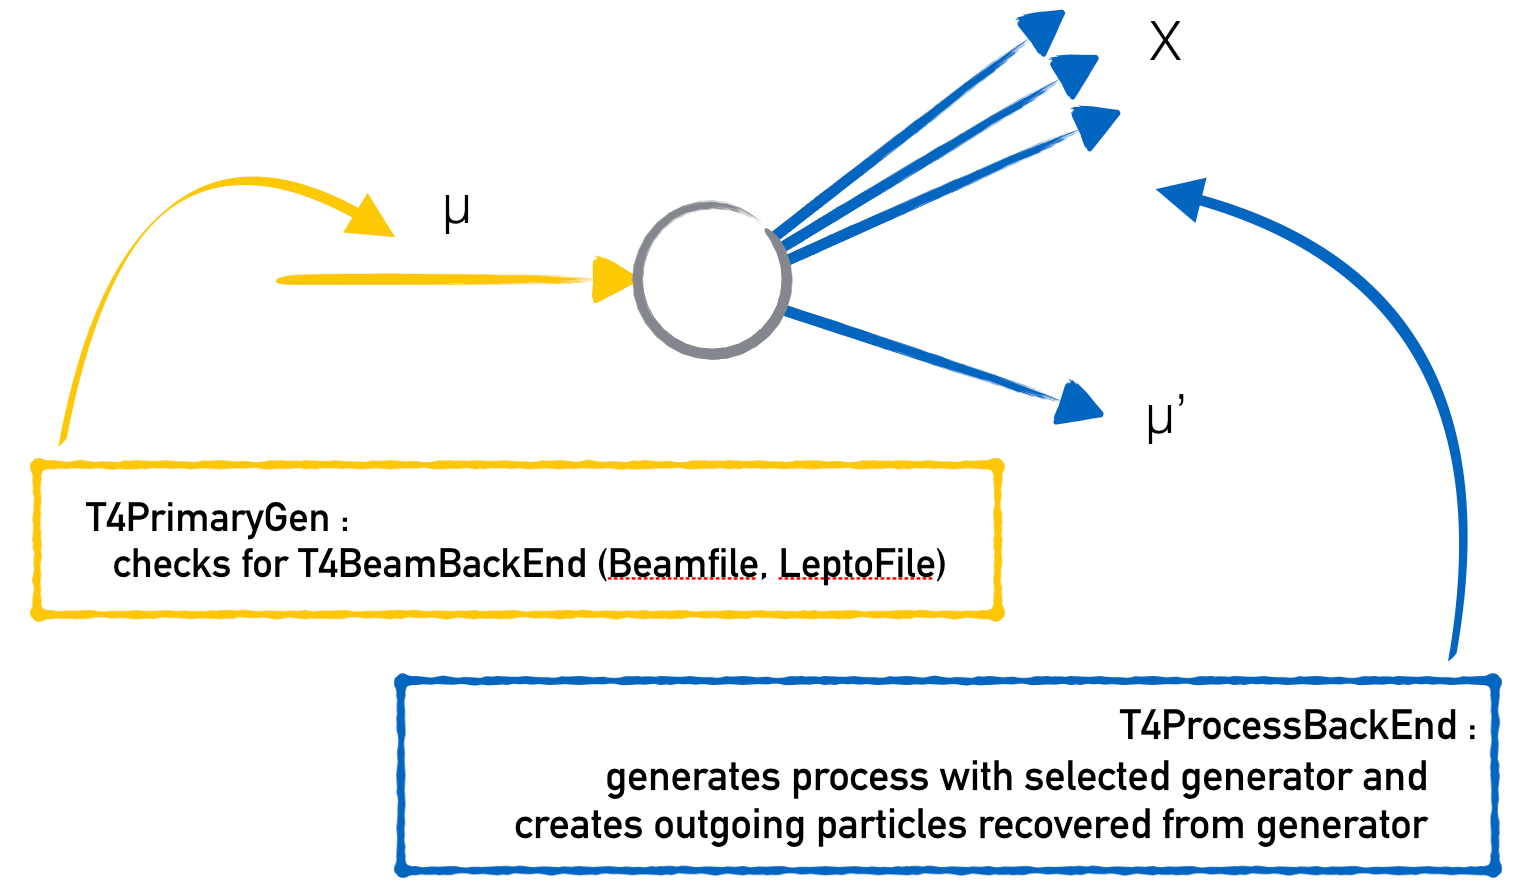
\epsfig{file=gfx/evtgenTG.png,width=11cm}}
\caption{Sketch showing how event generation is handled in TGEANT. A particle is first chosen in
the beamfile, then is sent to the dedicated generator that generates the given process. TGEANT then
recovers the list of particles from the generator, creates and propagates them.}\label{fig:evtgenTG}
\end{figure}
\newpage
There are two ways to implement a generator in TGEANT :
\begin{itemize}
\item As an internal generator (Pythia and HEPGEN++ way) : a C++ interface to the
generator is needed, the conservation of $P(p,E)$ is perfect and it only needs a
beamfile for the primary generator.
\item As an external generator (Lepto) : the beamfile is read by the standalone
generator, the primary generation and process infos are stored inside a file and
TGEANT has to do an extrapolation to -9 meters as the primary generation was done
outside of it, occasioning $P(p,E)$ being not perfectly conserved.
\end{itemize}

The external implementation is quite complicated as three classes are needed in order
to use the generator in TGEANT. First, the beamfile has to be read by the generator
which then outputs a file containing the beamfile infos but in its own format.
Then a first class has to be dedicated to the reading of the beamfile, recovering
the information about the selected muon in the file. A second class takes care of
passing of information between the generator and TGEANT. The last class is the
class of the generator itself (Fig. \ref{fig:leptoex}).

\begin{figure}[!htb]
\centerline{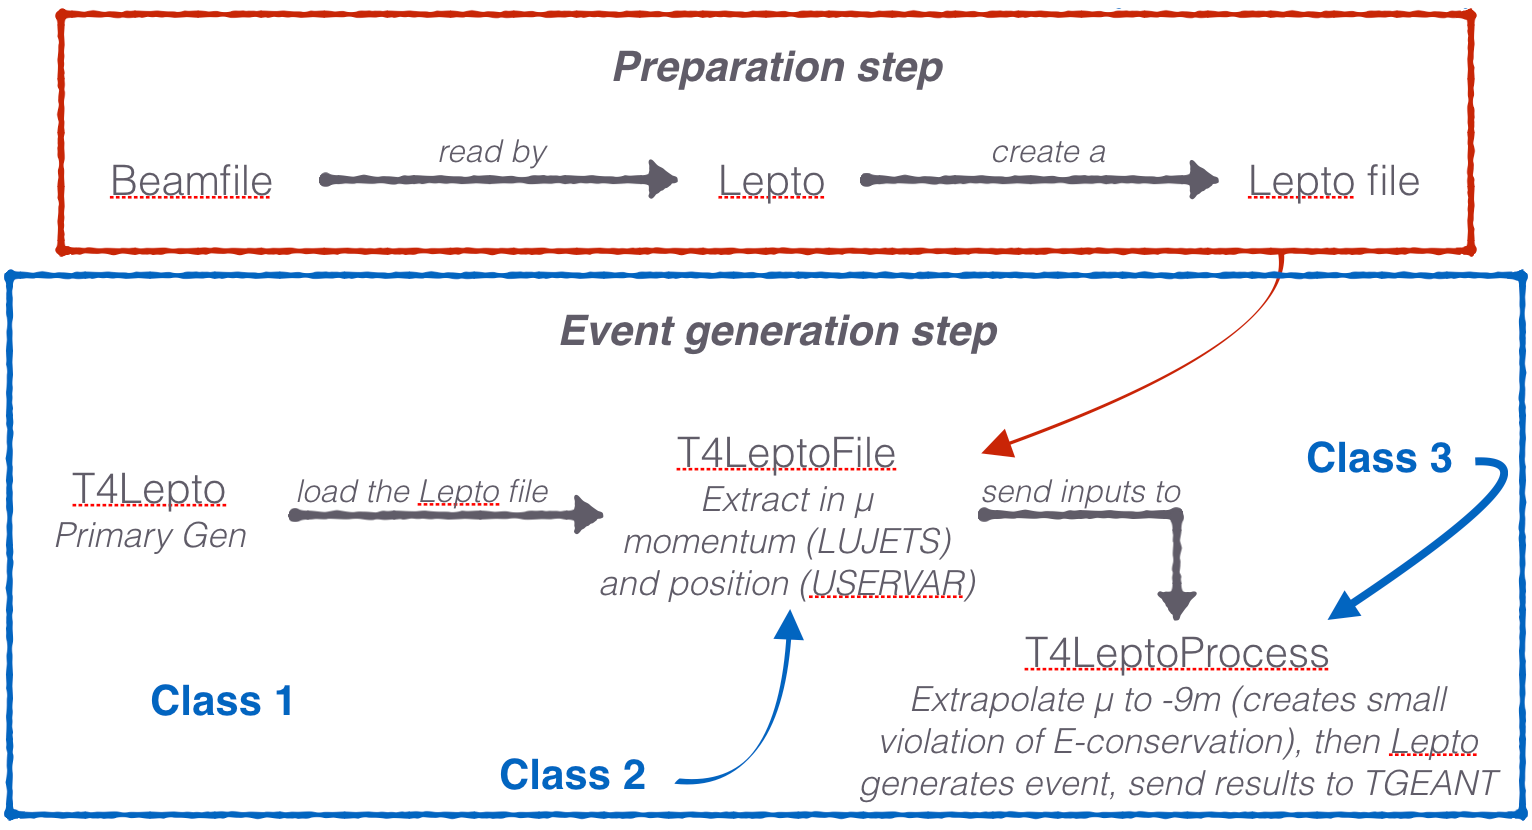
\epsfig{file=gfx/leptoex.png,width=12cm}}
\caption{Diagram explaining the philosophy of the external generator implementation, taking the
implementation of LEPTO as an example. First and foremost, a specific beamfile is created after the
initial one. The external generator will read this pregenerated file to extract infos about the incoming
particle. As these informations are at the interaction point, a backward propagation extrapolation in the
target material has to be made, inducing some small violations of energy conservation.
Then the generator is producing the event and sends the results to TGEANT.}\label{fig:leptoex}
\end{figure}

\newpage
If you apply this method to DJANGOH, then you encounter several critical problems :
\begin{itemize}
\item A new file format for the converted beamfile has to be created.
\item DJANGOH has to be modified to allow backward propagation of the incoming muon.
\item The result of fragmentation (LUJETS) has to be recovered in a file.
\end{itemize}
This results in many file accesses and consequently it is a non-efficient way to
implement DJANGOH inside TGEANT.

The internal implementation recquires perhaps more work on the generator itself however
this solution is much more efficient. Here, only two class are needed. One is the
interface class that creates instances of DJANGOH that can be manipulated in any C++
environment. This class is a C++ interface that is handling the FORTRAN part of DJANGOH.
The other class is taking care of passing the information between the interface to the
generator and TGEANT (Fig. \ref{fig:pythiaex}).

\begin{figure}[!htb]
\centerline{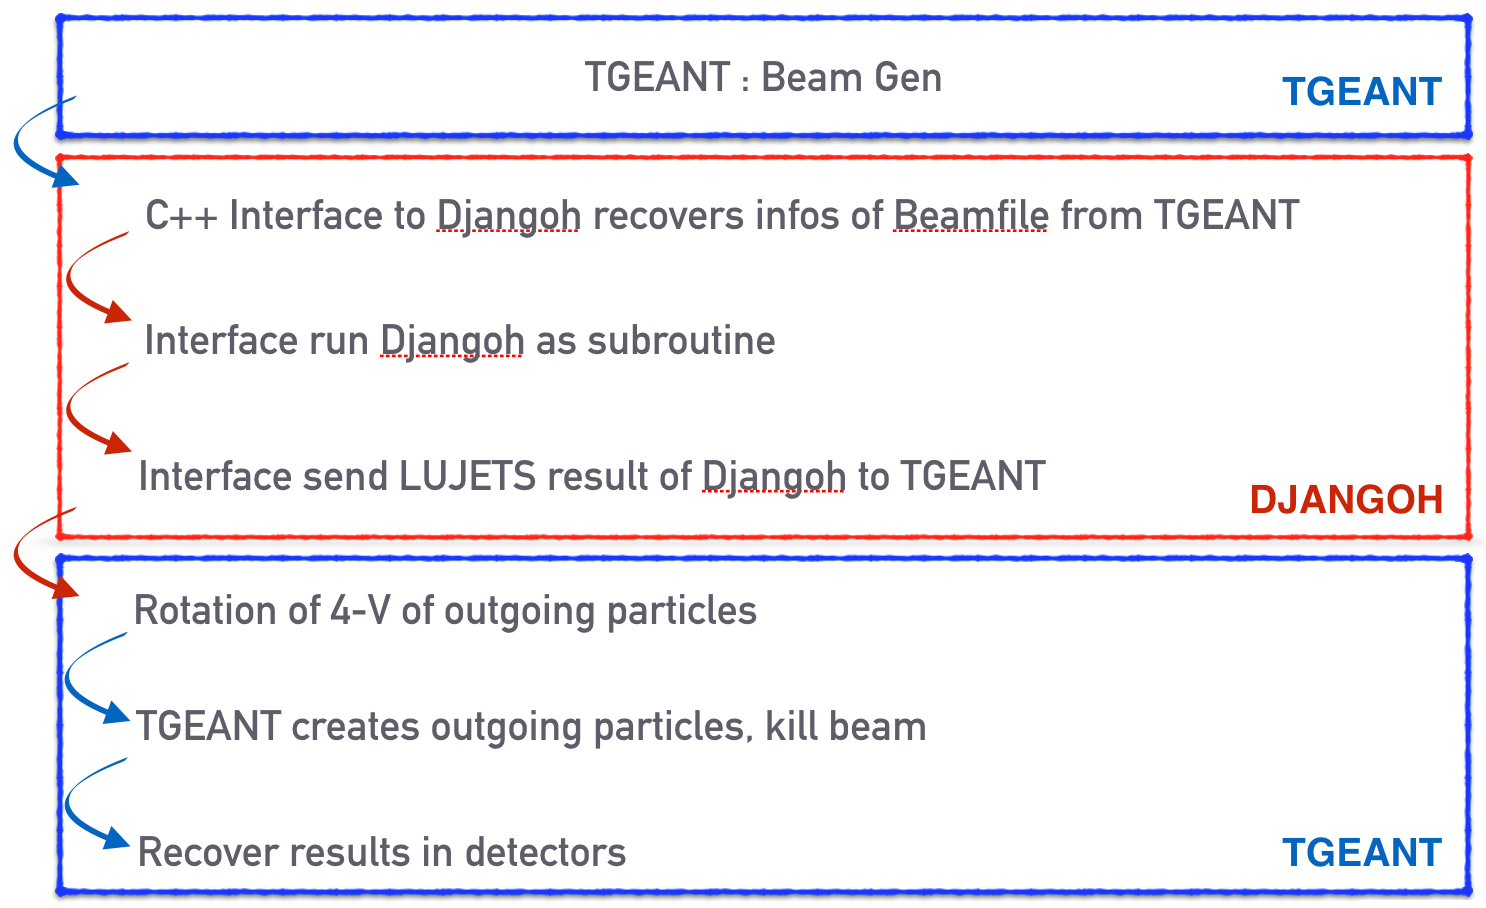
\epsfig{file=gfx/pythiaex.png,width=12cm}}
\caption{Diagram explaining the philosophy of the internal generator implementation.
The beamfile is read by TGEANT and the C++ interface to the generator is recovering the
informations of the incoming particle. This interface then runs the generator as a subroutine
and sends back the results of the generation to TGEANT, which then creates the outgoing particles
accordingly.}\label{fig:pythiaex}
\end{figure}

This second method was used to implement DJANGOH inside TGEANT.

%----------------------------------------------------------------------------------------

\section{Results on electroproduction from photon conversion}

Content
